\documentclass{standalone}

\usepackage[OT1]{fontenc}
\renewcommand*\familydefault{\sfdefault}
\usepackage{helvet,sfmath}
\usepackage{siunitx}

\usepackage{tikz}
\usetikzlibrary{arrows,calc,patterns}
\usepackage{tikz,tkz-euclide}


\definecolor{BlueDefault}{rgb}{0.2,0.2,0.7}

\begin{document}

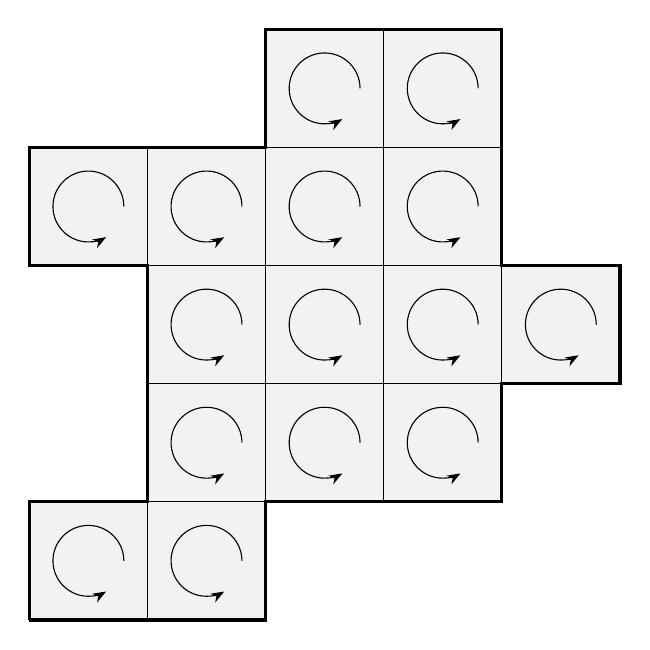
\begin{tikzpicture}[scale=1.5]
    \draw[very thick, fill = lightgray!20] (-2,-2) to (0,-2) to (0,-1) to (2,-1) to (2,0) to (3,0) to (3,1) to (2,1) to (2,3) to (0,3) to (0,2) to (-2,2) to (-2,1) to (-1,1) to (-1,-1) to (-2,-1) to (-2,-2);
    
    \foreach \x in {-1,0,1}
    { \foreach \y in {-1,0,1}
    {
    \draw (\x,\y) to (\x+1,\y) to (\x+1,\y+1) to (\x,\y+1) to (\x,\y);
    \draw[-Stealth] (\x+0.8,\y+0.5) arc (0:300:0.3);
    }
    }

    \foreach \x in {0,1}
    { \foreach \y in {2}
    {
    \draw (\x,\y) to (\x+1,\y) to (\x+1,\y+1) to (\x,\y+1) to (\x,\y);
    \draw[-Stealth] (\x+0.8,\y+0.5) arc (0:300:0.3);
    }
    }

    \foreach \x in {2}
    { \foreach \y in {0}
    {
    \draw (\x,\y) to (\x+1,\y) to (\x+1,\y+1) to (\x,\y+1) to (\x,\y);
    \draw[-Stealth] (\x+0.8,\y+0.5) arc (0:300:0.3);
    }
    }

    \foreach \x in {-1,-2}
    { \foreach \y in {-2}
    {
    \draw (\x,\y) to (\x+1,\y) to (\x+1,\y+1) to (\x,\y+1) to (\x,\y);
    \draw[-Stealth] (\x+0.8,\y+0.5) arc (0:300:0.3);
    }
    }

    \foreach \x in {-2}
    { \foreach \y in {1}
    {
    \draw (\x,\y) to (\x+1,\y) to (\x+1,\y+1) to (\x,\y+1) to (\x,\y);
    \draw[-Stealth] (\x+0.8,\y+0.5) arc (0:300:0.3);
    }
    }
\end{tikzpicture}    

\end{document}